% !TeX program = xelatex
% Build with XeLaTeX and the Windows Malgun Gothic font.
\documentclass[11pt,a4paper]{article}
\usepackage[margin=22mm]{geometry}
\usepackage{fontspec}
\setmainfont{Malgun Gothic}
\XeTeXlinebreaklocale "ko"
\XeTeXlinebreakskip=0pt plus 0.5pt
\usepackage{xcolor,amsmath,fancyvrb,graphicx}
\usepackage[hidelinks]{hyperref}
\definecolor{ink}{HTML}{152B42}
\definecolor{accent}{HTML}{185C67}
\setlength{\parindent}{0pt}
\setlength{\parskip}{5pt}
\raggedbottom
\newcommand{\api}[1]{\texttt{#1}}
\newcommand{\figurelabel}[1]{\refstepcounter{figure}{\small\textbf{Figure \thefigure.} #1}}
\newcommand{\partmark}[1]{\par\noindent{\large\color{accent}\bfseries #1}\par\smallskip}
\newcommand{\chaptermark}[1]{\par\noindent{\LARGE\color{ink}\bfseries #1}\par\smallskip}
\newcommand{\topic}[1]{\par\medskip{\large\color{accent}\bfseries #1}\par}
\DefineVerbatimEnvironment{Code}{Verbatim}{fontsize=\footnotesize,frame=leftline,framesep=6pt}
\hypersetup{pdftitle={DEVS in SOCS},pdfsubject={SOCS 시뮬레이션 모델 튜토리얼}}
\begin{document}

{\fontsize{34}{39}\selectfont\color{ink}\bfseries DEVS in SOCS}\par
{\large 예제로 배우는 Atomic, Coupled, 연속 상태 모델}\par
\vspace{3mm}{\color{accent}\hrule}\vspace{4mm}

SOCS 저장소 루트에서 Python 3.13 환경으로 실행합니다.
해당 환경에 SOCS를 설치하려면 먼저 \api{python -m pip install -e .}를 실행합니다.
라이브 창에는 Tkinter가 필요합니다. 라이브 phase 천이도를 보려면
Graphviz의 \api{dot}을 \api{PATH}에서 찾을 수 있거나
SOCS가 인식하는 Windows 기본 경로에 설치되어 있어야 합니다.

\partmark{Part 1 \enspace 이산 이벤트 시스템}
\chaptermark{Chapter 1 \enspace 시간 이벤트 시스템}
\begin{center}
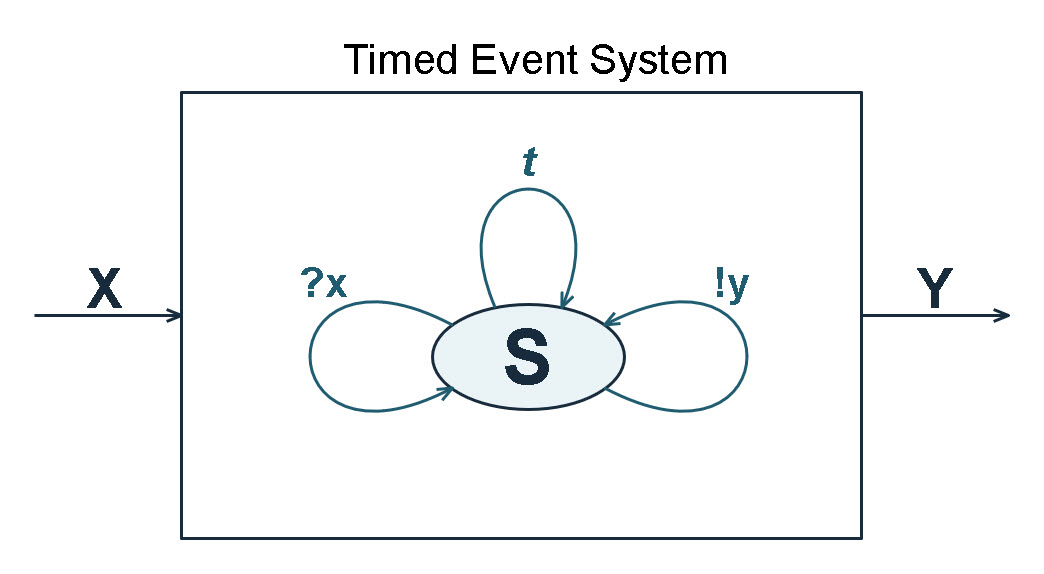
\includegraphics[width=.94\linewidth,height=10cm,keepaspectratio]{images/TimedEventSystem.jpg}\par
\figurelabel{시간 이벤트 시스템}
\end{center}
\begin{equation}
TES = (X, Y, S, s_0, \Delta_t, \Delta_x, \Delta_y)
\label{eq:tes}
\end{equation}
각 기호의 뜻은 다음과 같습니다.
\begin{itemize}
  \item $X$는 입력 이벤트의 집합입니다.
  \item $Y$는 출력 이벤트의 집합입니다.
  \item $S$는 상태의 집합입니다.
  \item $s_0 \in S$는 초기 상태입니다.
  \item $\Delta_t: S \times T \rightarrow S$는 연속 천이 함수입니다. 여기서 $T=[0,\infty)$는 시각을 나타내는 음이 아닌 실수의 집합입니다.
  \item $\Delta_x: S \times T \times X \rightarrow S$는 특정 시각에 입력 이벤트를 받았을 때 시스템의 상태가 어떻게 바뀌는지 정의하는 외부 천이 함수입니다.
  \item $\Delta_y: S \times T \rightarrow S\times Y$는 특정 시각에 시스템의 상태가 어떻게 바뀌고 어떤 출력 이벤트를 생성하는지 정의하는 내부 천이 함수입니다.
\end{itemize}

\newpage
\chaptermark{Chapter 2 \enspace DEVS}
\begin{center}
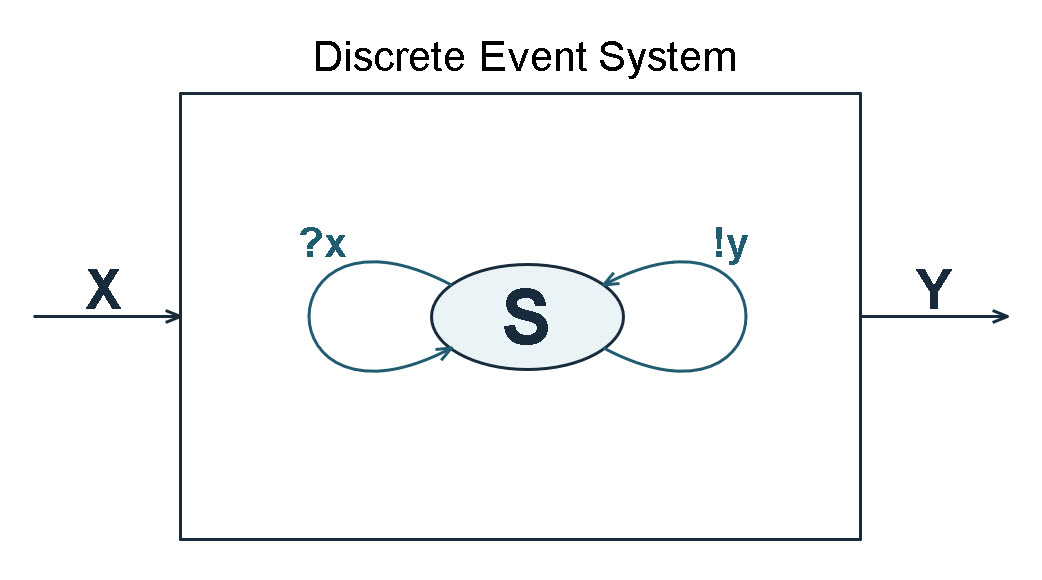
\includegraphics[width=.94\linewidth,height=10cm,keepaspectratio]{images/DEVS.jpg}\par
\figurelabel{DEVS}
\end{center}

\begin{equation}
DEVS=(X, Y, S, \delta_0, \delta_x, \delta_y, \tau)
\label{eq:devs}
\end{equation}

\newpage
\chaptermark{2.1 \enspace DEVS}

Atomic 모델은 자신의 상태와 천이를 정의합니다. Coupled 모델은 Atomic 모델이나
다른 Coupled 모델의 포트를 연결합니다. SOCS에서 이벤트는 \api{PortValue(port, value)}로
표현합니다. 포트 이름은 문자열이며, 전달할 값이 없으면 생략할 수 있습니다.

\topic{2.1.1 \enspace DEVSCounter}
\begin{Code}
python -m examples.DEVS_Simple.DEVSCounter --count 3
\end{Code}
\api{DEVSCounter.py}의 \api{Counter}를 살펴봅니다. \api{set\_initial\_state()}는 상태를
초기화하고, \api{tau()}는 다음 내부 이벤트까지의 시간을 반환합니다. 예약 시각에
\api{delta\_y()}가 현재 합계를 \api{!c}로 출력한 뒤 다음 정수를 더하고 카운트를
갱신합니다. 지정된 횟수를 세면 \(\tau=\infty\)인 Done으로 이동합니다.

\begin{Code}
def set_initial_state(self):
        """Initialize the counter state."""
        self.phase, self.count, self.sum = "C", 1, 0

def tau(self):
        """Return the time until the next internal event."""
        if self.phase == "C":
            return 5
        return float("inf")

def delta_x(self, event: PortValue) -> bool:
    """Ignore external events because this counter has no inputs."""
    return False

def delta_y(self) -> PortValue:
        """Emit the current sum, then update the counter state."""
        output = PortValue(self.OP["!c"], self.sum)
        if self.phase == "C":
            self.sum += self.count
            self.count += 1
            if self.count > self.count_no:
                self.phase = "D"
        return output
\end{Code}
모든 구체적인 \api{DEVS} 모델은 \api{set\_initial\_state()}, \api{tau()},
\api{delta\_x()}, \api{delta\_y()}를 구현합니다. 이 Counter의
\api{delta\_x()}는 입력을 무시하고 \api{False}를 반환합니다.

\begin{Code}
t=5  phase=Count count=1 sum=1 !c=0
t=10 phase=Count count=2 sum=3 !c=1
t=15 phase=Done  count=3 sum=6 !c=3
\end{Code}
\api{sum}은 갱신 후의 합계이고 \api{!c}는 바로 앞의 합계입니다.
\api{--live}를 붙이면 같은 시뮬레이션을 실행하면서 현재 phase와 남은 시간을 볼 수 있습니다.

\newpage
\chaptermark{2.1 \enspace DEVS (계속)}
\topic{2.1.2 \enspace DEVSToaster}
\begin{Code}
python -m examples.DEVS_Simple.DEVSToaster --live
\end{Code}
\textbf{Push}를 누르면 \api{?push} 입력을 전달합니다. 기본 가열 시간은 10초이며,
\api{--toasting-time 5}를 주면 5초로 바뀝니다. 콘솔 모드에서는 Enter로 가열을
시작하고 \api{q}로 종료합니다.

Idle에서 입력을 받으면 \api{delta\_x()}가 Toasting으로 이동하고 \api{True}를 반환합니다.
SOCS는 입력 시각에 새 phase의 \api{tau()}를 더해 다음 내부 이벤트를 예약합니다.
가열 중 다시 눌렀을 때는 \api{False}를 반환하므로 원래 완료 시각이 유지됩니다.
완료 시각에 \api{delta\_y()}가 \api{!pop}을 출력하고 Idle로 돌아갑니다.

\begin{Code}
def set_initial_state(self):
        """Reset the toaster to its initial idle phase."""
        self.phase = "Idle"

def tau(self):
        """Return the time until the next internal event."""
        if self.phase == "Toasting":
            return self.tt
        return inf

def delta_x(self, x):
        """Handle a push event and reschedule if toasting starts."""
        if isinstance(x, PortValue) and x.port == "?push" and self.phase == "Idle":
            self.phase = "Toasting"
            return True
        return False

def delta_y(self):
        """Emit the pop event and return to the idle phase."""
        if self.phase == "Toasting":
            self.phase = "Idle"
            return PortValue("!pop")
        return None
\end{Code}
콘솔에서 Enter를 눌렀을 때의 기본 10초 실행 결과입니다.
\begin{Code}
t=0 Idle> t=0 Toasting
t=10 Idle !pop
\end{Code}

\newpage
\chaptermark{2.1 \enspace DEVS (계속)}
\topic{2.1.3 \enspace DEVSPingPong}
\begin{Code}
python -m examples.DEVS_Simple.DEVSPingPong
\end{Code}
예제 메뉴에서 \api{s}를 선택하면 시뮬레이터로 들어갑니다.
A는 Sending에서 시작해 0.1 시간 단위 뒤에 공을 보냅니다.
B는 Waiting에서 시작하며 공을 받은 뒤 0.2 시간 단위가 지나면 돌려보냅니다.
두 선수 모두 \api{!s}로 공을 보내고 \api{?r}로 받습니다.

\begin{Code}
def set_initial_state(self):
        """Initialize the player's phase."""
        self.phase = self.initial_phase

def tau(self):
        """Return the time until the next internal event."""
        if self.phase == "S":
            return self.send_time
        return float("inf")

def delta_x(self, x):
        """Handle a received ball and request rescheduling when needed."""
        if x.port == "?r" and self.phase == "W":
            self.phase = "S"
            return True
        return False

def delta_y(self):
        """Send the ball and transition to the waiting phase."""
        if self.phase == "S":
            self.phase = "W"
            return PortValue(self.OP["!s"])
        return None
\end{Code}
\begin{Code}
model.addOutputPorts("!ping", "!pong")
model.addCouples(
    ((player_a, "!s"), (player_b, "?r")),
    ((player_b, "!s"), (player_a, "?r")),
    ((player_a, "!s"), (model, "!ping")),
    ((player_b, "!s"), (model, "!pong")),
)
\end{Code}
연결의 양 끝은 각각 (모델, 포트 이름)입니다.
A의 출력은 B와 Coupled 모델의 경계 포트 \api{!ping}으로 전달됩니다.
B의 출력은 A와 \api{!pong}으로 전달됩니다.
두 경계 출력은 \(t=0.1,\ 0.3,\ 0.4,\ 0.6,\ldots\)에서 번갈아 발생합니다.

\begin{Code}
t=0.1  !ping
t=0.3  !pong
t=0.4  !ping
t=0.6  !pong
\end{Code}
\topic{라이브 화면의 역할}
화면은 입력을 엔진에 전달하고, 엔진이 시뮬레이션을 한 단계 진행하면 갱신된
모델 상태를 그립니다. 모델 클래스에서 동작을 정의하고, 라이브 화면에서 그
동작의 결과를 확인할 수 있습니다.

\newpage
\chaptermark{2.2 \enspace DEVSph}
\begin{equation}
DEVS_{ph}=(X, Y, S_{p}, \delta_{0,p}, \delta_{0,p}, \delta_{0,p})
\label{eq:devsph}
\end{equation}

DEVSph와 cDEVSph 예제는 기본으로 라이브 창을 엽니다. \api{--live}로 명시해도 같고, 텍스트 실행은 \api{--console}을 사용합니다.

\api{DEVSph}에서는 phase 그래프를 선언합니다. 정점에는 phase 이름과 \api{tau}가,
방향 간선에는 내부 또는 외부 천이가 들어갑니다. SOCS는 선언된 \api{AGraph}에서
실행할 천이를 고르고, 라이브 화면은 같은 그래프를 읽어 천이도를 그립니다.

\topic{2.2.1 \enspace DEVSphToaster}
\begin{Code}
python -m examples.DEVS_Simple.DEVSphToaster --live
\end{Code}
외부 이벤트 입력 패널에서 모델 \api{Toaster}와 포트 \api{?push}를 고릅니다.
\textbf{Value (JSON)}을 비우고 \textbf{Apply}를 누르면 Python \api{None}이 전달됩니다.
모델에는 다음 phase와 천이가 선언되어 있습니다.

\begin{Code}
self.add_phase("Idle", tau=inf, initial=True)
self.add_phase("Toasting", tau=toasting_time)
self.add_external_transition(
    "Idle", "Toasting", input_port="?push", reschedule=True,
)
self.add_internal_transition("Toasting", "Idle", output="!pop")
\end{Code}
\api{?push} 간선은 Idle에서만 출발합니다. Toasting에서 같은 입력을 받아도
상태와 완료 예약이 유지되므로 그림에 자기 루프가 없습니다.
\textbf{DEVS Only}에서는 Apply로 외부 이벤트를 전달하고,
\textbf{Step}으로 다음 내부 이벤트 하나를 실행합니다.
\textbf{Animation}에서는 가열 중 0.1 시뮬레이션 초마다 화면을 갱신합니다.

\topic{천이도 읽기}
진입 화살표는 초기 phase를 가리킵니다. 색으로 강조된 현재 phase에서
\(t_{\mathrm{next}}-t_{\mathrm{now}}\)를 남은 시간으로 표시합니다.
\(\tau=\infty\)인 phase의 테두리는 점선입니다.
내부 천이와 \api{reschedule=True}인 외부 천이는 실선이고,
\api{reschedule=False}인 외부 천이는 점선입니다. 점선 자기 루프는
phase와 예약 시각을 유지하면서 모델 데이터를 갱신하는 천이를 나타낼 수 있습니다.

\begin{center}
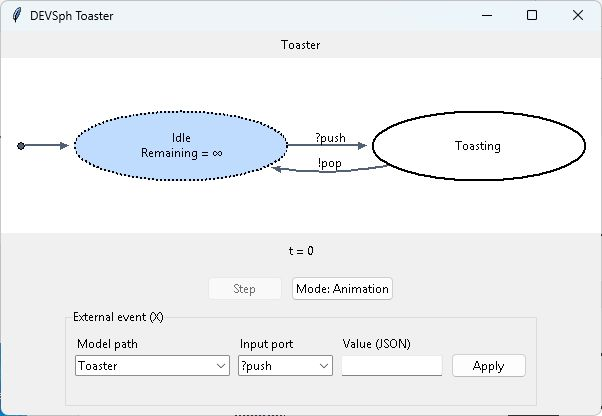
\includegraphics[width=.92\linewidth,height=6.7cm,keepaspectratio]{images/toaster.jpg}\par
\figurelabel{Toaster의 기본 입력 대상. Value는 비우고 Apply를 누릅니다.}
\end{center}

\newpage
\chaptermark{2.2 \enspace DEVSph (계속)}
\topic{2.2.2 \enspace DEVSphPingPong}
\begin{Code}
python -m examples.DEVS_Simple.DEVSphPingPong --live
\end{Code}
천이도에 각 선수의 계층 경로인 \api{PingPong.A}, \api{PingPong.B}가 표시됩니다.
\textbf{Show Coupling}을 누르면 전체 연결 네 개를 볼 수 있습니다.
Animation 간격은 0.01 시뮬레이션 시간 단위입니다.
DEVS Only에서는 Step마다 송신이 한 번 일어납니다.
\api{--console --steps 4}를 주면 송신 네 번을 출력합니다.

\begin{Code}
self.addInputPorts("?r")
self.addOutputPorts("!s")
self.add_phase("Sending", tau=send_time, initial=starts)
self.add_phase("Waiting", tau=inf, initial=not starts)
self.add_external_transition(
    "Waiting", "Sending", input_port="?r", reschedule=True,
)
self.add_internal_transition("Sending", "Waiting", output="!s")
\end{Code}
입력 패널에서 \api{PingPong.B}와 \api{?r}를 고르고 값은 비울 수 있습니다. Apply는 현재 시각에 공을 받은 것과 같은 외부 이벤트를 보냅니다. Waiting에서만 수신 천이가 활성화됩니다. 기본 왕복 시각을 비교할 때는 추가 입력 없이 실행합니다.
\begin{center}
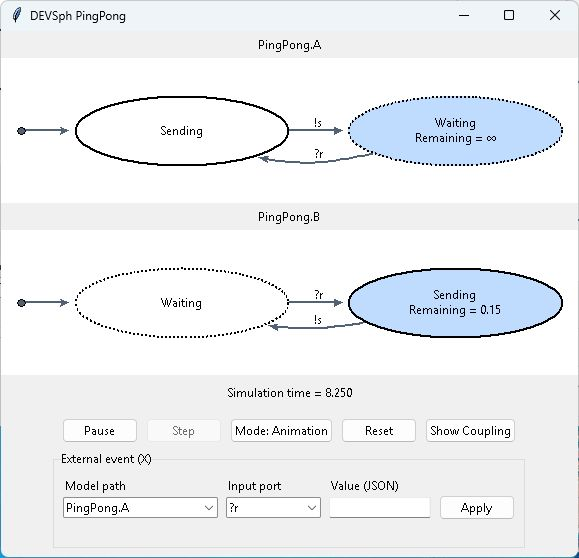
\includegraphics[width=.92\linewidth,height=8.3cm,keepaspectratio]{images/pingpong.jpg}\par
\figurelabel{두 선수의 phase, 실행 모드, coupling 버튼과 외부 이벤트 입력.}
\end{center}

\newpage
\chaptermark{2.2 \enspace DEVSph (계속)}
\topic{2.2.3 \enspace DEVSphCounterBasic}
\begin{Code}
python -m examples.DEVS_Simple.DEVSphCounterBasic --live --count 3
\end{Code}
CounterBasic은 전체 상태 하나마다 그래프 정점 하나를 둡니다.
정점 이름에는 phase, 완료 횟수, 누적 합계가 들어갑니다.
\begin{equation}
 \mathrm{Count}(0,0)\ \longrightarrow\
 \mathrm{Count}(1,1)\ \longrightarrow\
 \mathrm{Count}(2,3)\ \longrightarrow\
 \mathrm{Done}(3,6)
\label{eq:counter-states}
\end{equation}
각 Count 정점의 시간 전진값은 5이고 내부 천이는 하나씩 있습니다.
간선에는 \api{PortValue("!c", 0)}처럼 고정 출력을 지정할 수 있습니다.
도착 정점에 갱신된 횟수와 합계가 들어 있으므로 \api{guard}와 \api{action} 없이
동작을 선언할 수 있습니다.

아래는 생성 루프가 등록하는 첫 두 정점과 첫 간선을 풀어 쓴 코드입니다.
\begin{Code}
self.addOutputPorts("!c")
self.add_phase("Count(0, 0)", tau=5, initial=True)
self.add_phase("Count(1, 1)", tau=5)
self.add_internal_transition(
    "Count(0, 0)", "Count(1, 1)", output=PortValue("!c", 0),
)
\end{Code}
\begin{center}
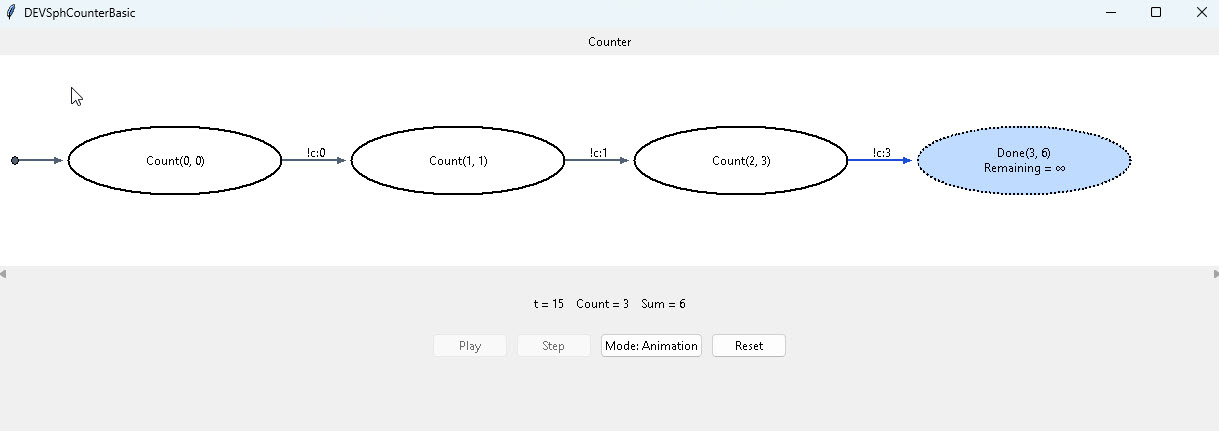
\includegraphics[width=.92\linewidth,height=7.5cm,keepaspectratio]{images/counter_basic.jpg}\par
\figurelabel{완료 시점에는 마지막 정점 쪽으로 이동합니다. 아래 스크롤 막대로 앞쪽 정점을 볼 수 있습니다.}
\end{center}

\newpage
\chaptermark{2.2 \enspace DEVSph (계속)}
\topic{2.2.4 \enspace DEVSphCounter}
\begin{Code}
python -m examples.DEVS_Simple.DEVSphCounter --live --count 3
\end{Code}
같은 카운터를 Count와 Done 두 phase로 표현할 수 있습니다. 완료 횟수와 누적
합계는 \api{self.\_variable}에 저장합니다. Count에서 출발하는 내부 천이는 두 개입니다.

\begin{Code}
self.addOutputPorts("!c")
self.add_phase("Count", tau=5, initial=True)
self.add_phase("Done", tau=inf)
self.add_internal_transition(
    "Count", "Count", guard=self.has_more_ticks,
    action=self.increment, output=self.emit_sum,
)
self.add_internal_transition(
    "Count", "Done", guard=self.is_last_tick,
    action=self.increment, output=self.emit_sum,
)
\end{Code}
\api{guard(model, event)}는 해당 간선을 실행할 수 있는지 판단합니다.
\api{action(model, event)}은 선택된 간선에서 상태를 갱신합니다. 내부 천이에서
\api{event}는 \api{None}입니다. 활성화된 간선 하나를 고른 뒤 출발 상태로 출력을
만들고, action을 실행한 다음 목적 phase로 이동합니다. 천이도는 각 간선의
guard와 action 함수 이름을 표시합니다.

\begin{Code}
@staticmethod
def has_more_ticks(model, event):
    return model._variable.count + 1 < model.count_no

@staticmethod
def is_last_tick(model, event):
    return not model.has_more_ticks(model, event)

@staticmethod
def increment(model, event):
    model._variable.count += 1
    model._variable.sum += model._variable.count
\end{Code}

세 번째 이벤트에서는 \api{is\_last\_tick}에 의해 Count에서 Done으로 이동합니다.
\api{emit\_sum}이 3을 출력한 뒤 \api{increment}가 횟수를 3, 합계를 6으로 갱신합니다.
두 예제를 DEVS Only로 실행해 2.1.1의 이벤트 시각과 출력 순서와 비교해 보세요.

두 Counter에는 입력 포트가 없습니다. Play/Pause, Step, Mode, Reset으로 실행을 제어합니다.
\begin{center}
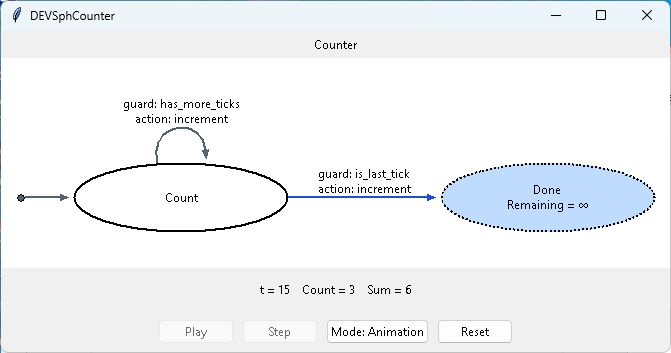
\includegraphics[width=.92\linewidth,height=5.1cm,keepaspectratio]{images/counter.jpg}\par
\figurelabel{Count의 두 간선에 guard와 action 이름이 표시됩니다.}
\end{center}

\newpage
\partmark{Part 2 \enspace 연속 및 이산 이벤트 시스템}
\chaptermark{Chapter 3 \enspace 연속 및 이산 이벤트 시스템}
\begin{center}
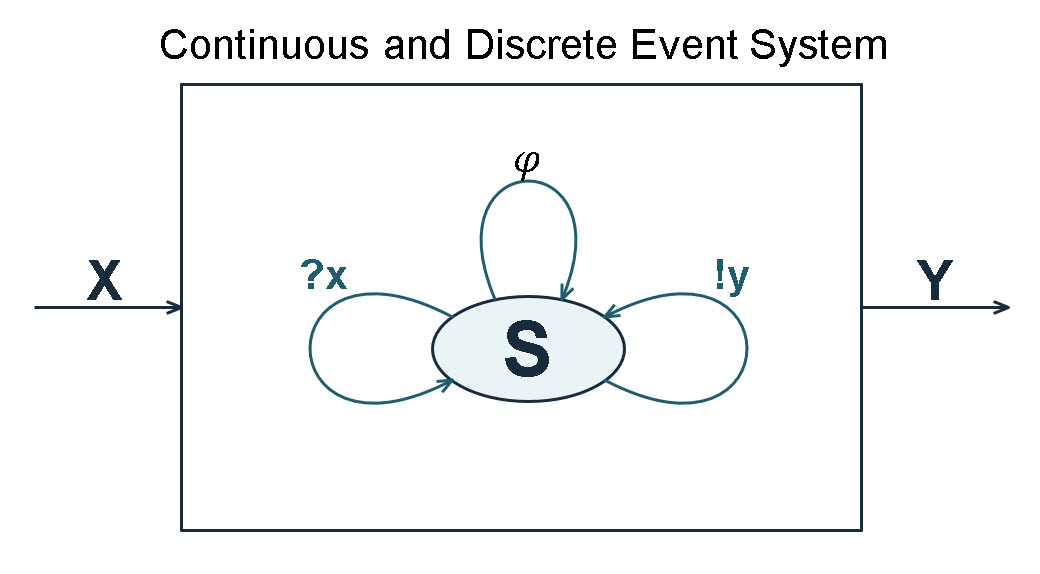
\includegraphics[width=.94\linewidth,height=10cm,keepaspectratio]{images/CDEVS.jpg}\par
\figurelabel{연속 및 이산 이벤트 시스템}
\end{center}

\newpage
\chaptermark{cDEVS and cDEVSph}

\api{cDEVS}는 모델에 \api{delta\_cont(elapsed)}를 추가합니다.
\api{cDEVSph}는 여기에 phase 그래프를 결합합니다.
엔진은 새 시뮬레이션 시각에 도착하면 이벤트를 처리하기 전에
\api{Delta\_null(t)}을 호출합니다. 연속 모델은 현재 phase의 운동 규칙을
경과 시간에 적용합니다. 같은 시각에 여러 이벤트가 있어도 시간 갱신은 한 번
이루어집니다. 유한 종료 시각에도 모델을 해당 시각까지 전진시킵니다.

\topic{cDEVSphElevator}
\begin{Code}
python -m examples.DEVS_Simple.cDEVSphElevator --live
\end{Code}
승강기는 1층에서 시작합니다. 모델 \api{Elevator}, 입력 포트 \api{?floor},
JSON 값 \api{2}를 선택하고 Apply를 누르면 2층으로 올라갑니다.
도착 후 값 \api{1}을 보내면 내려옵니다. 층 번호는 따옴표 없이 입력합니다.
\api{--console}에서는 왕복을 실행하고 각 phase 경계의 상태를 출력합니다.

\begin{equation}
 \mathrm{Idle}\ \longrightarrow\ \mathrm{Accelerating}\
 \longrightarrow\ \mathrm{Cruising}\ \longrightarrow\
 \mathrm{Braking}\ \longrightarrow\ \mathrm{Idle}
\label{eq:elevator-phases}
\end{equation}
층간 거리는 3 m입니다. 0.5초 동안 가속하고, 1.5 m/s로 1.5초 동안
등속 이동한 뒤 0.5초 동안 감속합니다. 첫 이동의 phase 경계는
\(t=0.5,\ 2.0,\ 2.5\)초입니다. 마지막 내부 천이는 목표 층 번호를
\api{!arrived}로 출력합니다.

\begin{Code}
self.add_phase("Idle", tau=inf, initial=True)
self.add_phase("Accelerating", tau=self.RAMP_TIME)
self.add_phase("Cruising", tau=self.FLOOR_HEIGHT / self.TOP_SPEED
               - self.RAMP_TIME)
self.add_phase("Braking", tau=self.RAMP_TIME)
self.add_external_transition(
    "Idle", "Accelerating", input_port="?floor", reschedule=True,
    match=lambda floor: type(floor) is int and floor in (1, 2),
    guard=self.is_different_floor, action=self.set_target,
)
self.add_internal_transition("Accelerating", "Cruising")
self.add_internal_transition("Cruising", "Braking")
self.add_internal_transition(
    "Braking", "Idle", action=self.finish_trip,
    output=lambda model: PortValue("!arrived", model._variable.target),
)
\end{Code}

층 번호 검사 후 guard는 현재 층과 목표 층이 다른지 확인합니다. 첫 action은 목표 층을 저장하고, 도착 action은 현재 층, 위치, 속도를 갱신합니다.
\begin{Code}
@staticmethod
def is_different_floor(model, event):
    return event.value != model._variable.floor

@staticmethod
def set_target(model, event):
    model._variable.target = event.value

@staticmethod
def finish_trip(model, event):
    target = model._variable.target
    model._variable.update(
        floor=target, position=(target - 1) * model.FLOOR_HEIGHT,
        velocity=0.0,
    )
\end{Code}

\newpage
\chaptermark{cDEVS and cDEVSph (계속)}
\topic{phase 안에서 변하는 위치와 속도}
\api{tNow}는 상태를 계산할 현재 시뮬레이션 시각입니다.
\api{tLast}는 모델의 예약 기준 시각이며, 이 엘리베이터에서는 현재 phase의 시작 시각입니다.
\(t=0\)에 가속을 시작했다면 \(t=0.10\)의 화면 갱신에서 \api{tNow}는 0.10이고
\api{tLast}는 여전히 0입니다. 따라서 경과 시간은
\(\Delta t=\api{tNow}-\api{tLast}=0.10\)초입니다.

가속도 \(a\)가 일정할 때 \api{delta\_cont()}는 phase 시작 위치 \(x_L\)과
속도 \(v_L\)을 기준으로 현재 위치와 속도를 계산합니다.
\begin{equation}
 x(t) = x_L+v_L\Delta t+\tfrac12 a(\Delta t)^2,\qquad
 v(t) = v_L+a\Delta t .
\label{eq:elevator-motion}
\end{equation}
이동 방향에 따라 속도와 가속도의 부호가 달라집니다. 도착하면 목표 층에 위치하고
속도는 0이 됩니다.

\begin{Code}
def delta_cont(self, elapsed):
    """Evaluate motion at elapsed seconds after the current phase began."""
    if self.phase == "Idle":
        return
    state = self._variable
    direction = state.target - state.floor
    start = (state.floor - 1) * self.FLOOR_HEIGHT
    ramp_distance = self.TOP_SPEED * self.RAMP_TIME / 2
    acceleration = self.TOP_SPEED / self.RAMP_TIME
    if self.phase == "Accelerating":
        distance = acceleration * elapsed**2 / 2
        speed = acceleration * elapsed
    elif self.phase == "Cruising":
        distance = ramp_distance + self.TOP_SPEED * elapsed
        speed = self.TOP_SPEED
    else:
        distance = (self.FLOOR_HEIGHT - ramp_distance
                    + self.TOP_SPEED * elapsed)
        distance -= acceleration * elapsed**2 / 2
        speed = self.TOP_SPEED - acceleration * elapsed
    state.position = start + direction * distance
    state.velocity = direction * speed
\end{Code}
같은 phase에서 화면이 여러 번 갱신돼도 같은 시작점을 기준으로 계산합니다.
phase 전환과 \api{!arrived} 출력은 이산 천이가 처리합니다.
\topic{같은 시뮬레이션을 보는 두 화면}
천이도는 현재 phase와 남은 시간을 보여 줍니다. 승강로는 같은 모델의 위치를
미터에서 픽셀로 변환해 그립니다. 화면 코드는 \api{\_elevator\_view.py}에 있습니다.

\begin{center}
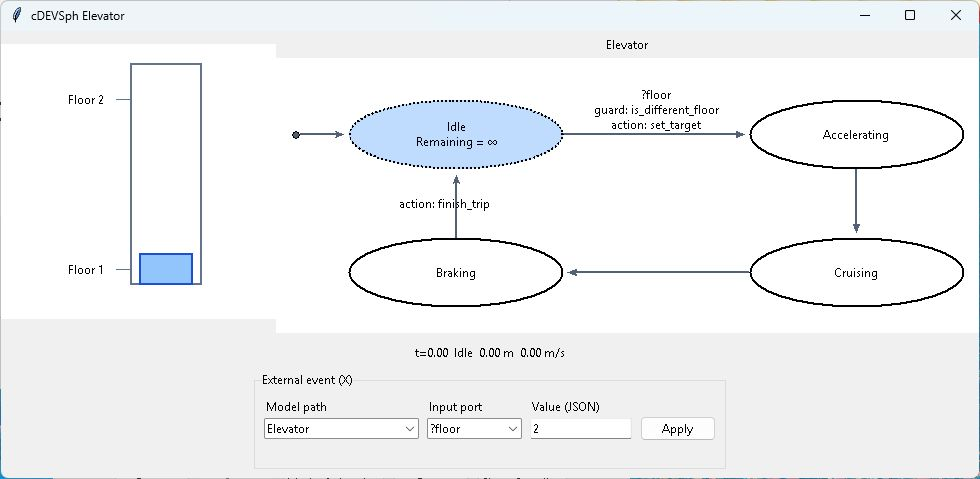
\includegraphics[width=.92\linewidth,height=5.4cm,keepaspectratio]{images/elevator.jpg}\par
\figurelabel{1층에서 대기 중인 승강기. 입력값 2를 보내면 가속 phase로 이동합니다.}
\end{center}

\end{document}
